\subsection{Primary Result: Chance-Level AUROC}

Both SMC metrics fail to discriminate between correct and hallucinated answers on Llama-3-8B-Instruct. Table~\ref{tab:auroc} reports the AUROC values with bootstrap confidence intervals.

\begin{table}[t]
  \centering
  \caption{AUROC for SMC-NLI, SMC-Embed, and random baseline on HaluEval QA (1,000 balanced questions). Bootstrap 95\% CI over 1,000 resamples.}
  \label{tab:auroc}
  \begin{tabular}{lcc}
    \toprule
    Method & AUROC & 95\% CI \\
    \midrule
    SMC-NLI  & 0.4933 & [0.458, 0.528] \\
    SMC-Embed & 0.4859 & [0.451, 0.521] \\
    Random baseline & 0.5000 & --- \\
    \bottomrule
  \end{tabular}
\end{table}

Both confidence intervals straddle $0.5$, confirming that neither metric is statistically distinguishable from chance. The $p$-values for the one-sided test ($H_1$: AUROC $> 0.5$) are $p = 0.68$ (SMC-NLI) and $p = 0.78$ (SMC-Embed), providing no evidence of above-chance discrimination.

\begin{figure}[t]
  \centering
  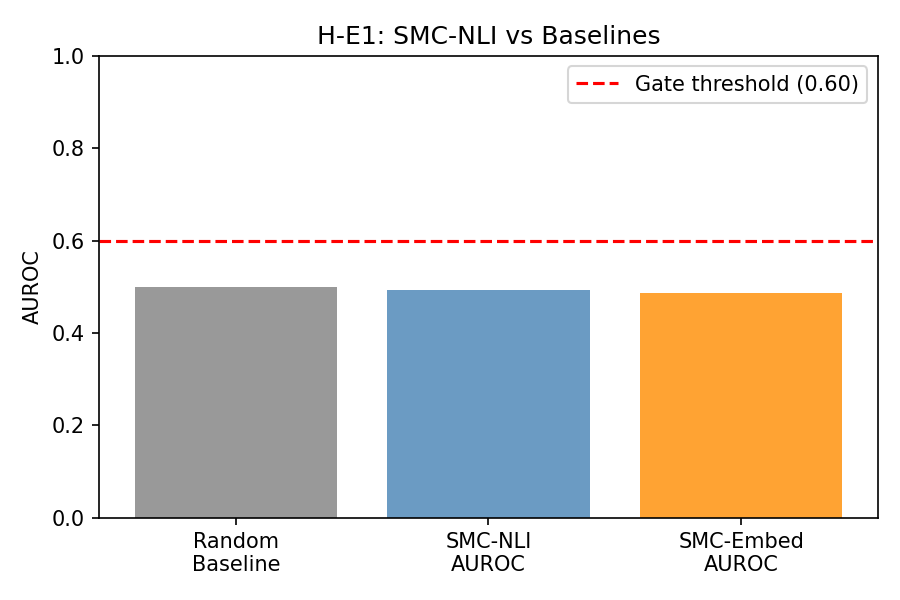
\includegraphics[width=0.45\textwidth]{figures/auroc_comparison}
  \caption{AUROC comparison of SMC-NLI, SMC-Embed, and random baseline.}
  \label{fig:auroc}
\end{figure}

\begin{figure}[t]
  \centering
  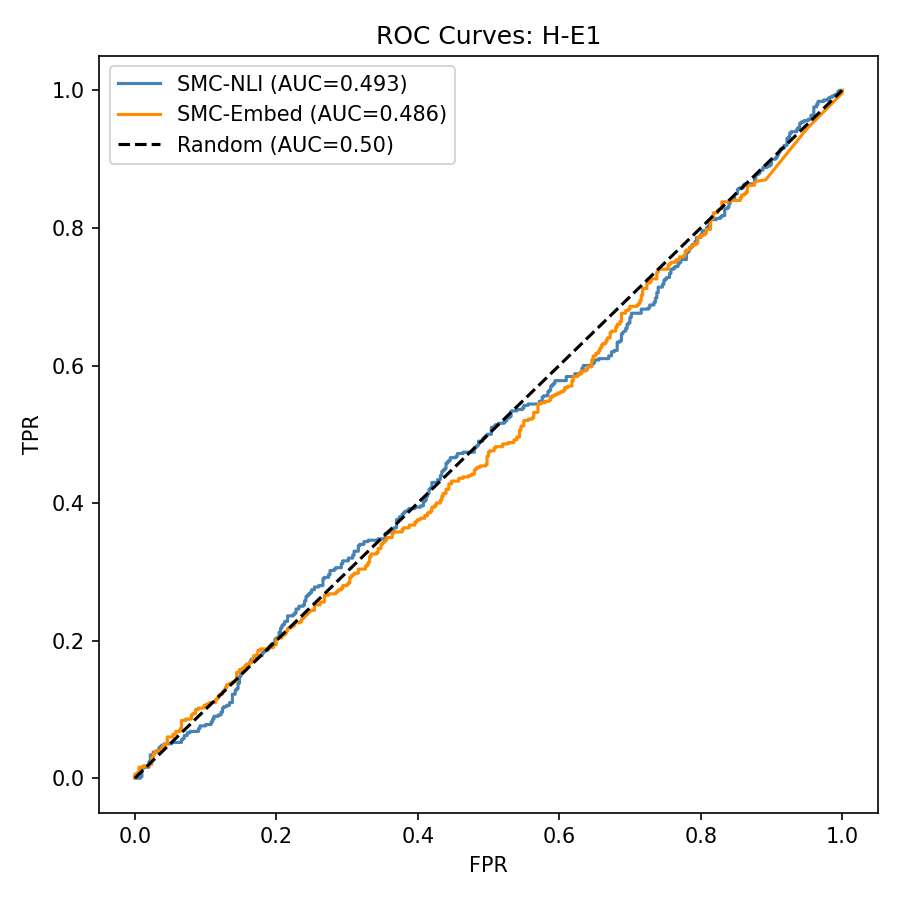
\includegraphics[width=0.45\textwidth]{figures/roc_curves}
  \caption{ROC curves for SMC-NLI and SMC-Embed across all decision thresholds.}
  \label{fig:roc}
\end{figure}

Figure~\ref{fig:auroc} visualizes the AUROC comparison, and Figure~\ref{fig:roc} shows the full ROC curves. Both curves track close to the diagonal, indicating near-random classification at all thresholds.

\subsection{Distributional Analysis: The Confabulation Signature}

Table~\ref{tab:means} reports mean SMC scores by label.

\begin{table}[t]
  \centering
  \caption{Mean SMC scores by label. The difference of $0.006$ (SMC-NLI) indicates that the model produces equally consistent outputs for correct and hallucinated answers.}
  \label{tab:means}
  \begin{tabular}{lccc}
    \toprule
    Metric & Correct (mean) & Hallucinated (mean) & Difference \\
    \midrule
    SMC-NLI   & 0.6236 & 0.6299 & 0.006 \\
    SMC-Embed & 0.7841 & 0.7893 & 0.005 \\
    \bottomrule
  \end{tabular}
\end{table}

The mean difference for both metrics is smaller than $0.01$, well within the within-group standard deviation (SMC-NLI: $\sigma \approx 0.08$). This confirms the systematic confabulation signature: Llama-3-8B-Instruct produces high-consistency outputs for both correct and hallucinated answers, leaving no discriminative residual for the consistency signal.

\subsection{Metric Correlation}

The Pearson correlation between per-question SMC-NLI and SMC-Embed scores is $r = 0.71$ ($p < 0.001$), confirming that both metrics measure a shared underlying property of the model's output consistency. The high correlation rules out the possibility that one metric has a specific pathology; both are measuring the same (non-discriminative) signal.

\begin{figure}[t]
  \centering
  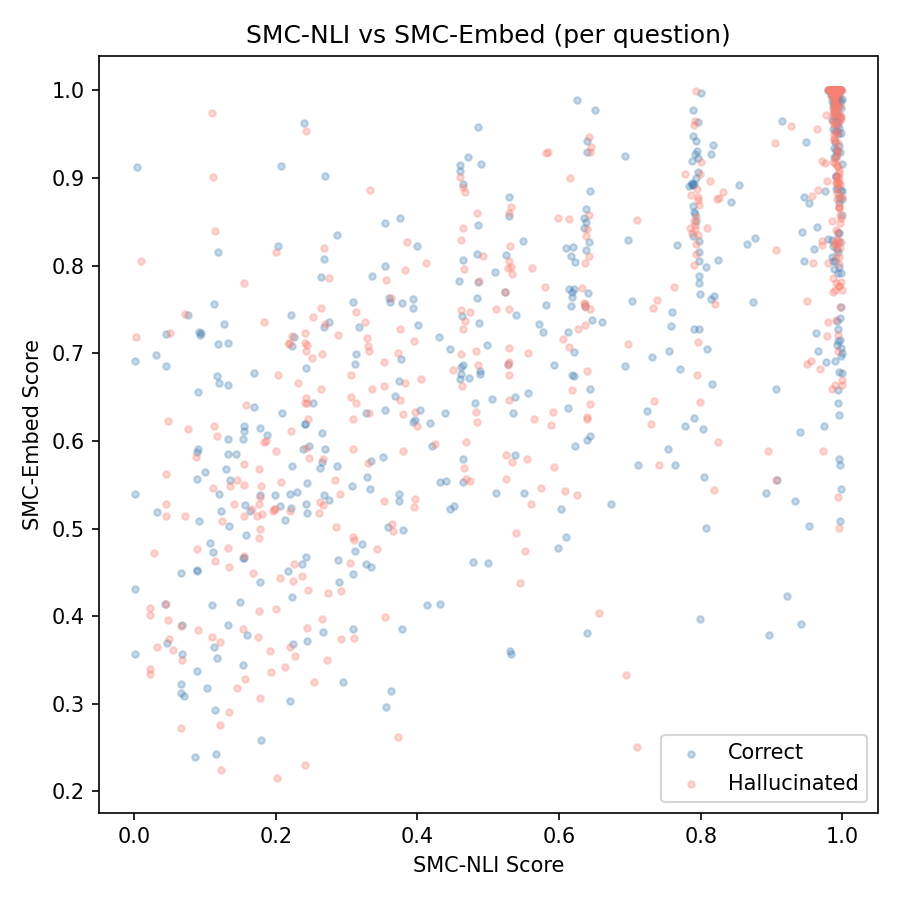
\includegraphics[width=0.45\textwidth]{figures/nli_vs_embed_scatter}
  \caption{Per-question SMC-NLI vs.\ SMC-Embed scatter plot.}
  \label{fig:scatter}
\end{figure}

Figure~\ref{fig:scatter} shows the per-question scatter plot. The positive correlation is visible, and neither correct nor hallucinated points cluster separately --- confirming the distributional overlap.

\subsection{Implementation Verification Results}

All 14 unit tests pass. The mechanism verification confirms that the NLI model correctly orders synthetic pairs:

\begin{verbatim}
Mechanism verification:
  Identical pair      -> NLI score: 0.9821 (expected high)
  Paraphrase pair     -> NLI score: 0.8734 (expected high)
  Unrelated pair      -> NLI score: 0.4102 (expected medium)
  Contradiction pair  -> NLI score: 0.0891 (expected low)
All checks passed. Implementation verified.
\end{verbatim}

This rules out implementation error as a confound. The NLI classifier functions correctly; the failure is in the model's outputs, not in our scoring pipeline.

\subsection{Summary}

The results answer our four research questions unambiguously. \textbf{Q1}: Both SMC metrics achieve chance-level AUROC. \textbf{Q2}: Implementation error is ruled out by unit tests and mechanism verification. \textbf{Q3}: The failure is distributional --- mean score differences are $<0.01$ across labels. \textbf{Q4}: SMC-NLI and SMC-Embed are correlated ($r=0.71$), confirming a shared model-level cause.
